\documentclass[conference]{IEEEtran}
\usepackage[T1]{fontenc}
\usepackage{amsmath,amssymb,booktabs,array}
\usepackage{algorithm,algpseudocode}
\usepackage{tikz}
\usetikzlibrary{arrows.meta,positioning}
\usepackage[hidelinks]{hyperref}
\usepackage{url,cite}
\pagestyle{plain}
\newcommand{\code}[1]{\texttt{#1}}
\newcommand{\smalltable}{\fontsize{8}{9.5}\selectfont}
\title{Safe Recovery After an Agent Skill Is Blocked:\\An Empirical Study of Mechanisms and Their Limits}
\author{\IEEEauthorblockN{Victor Cao}\IEEEauthorblockA{University of Auckland\\Auckland, New Zealand\\xcao541@aucklanduni.ac.nz}\and\IEEEauthorblockN{Enlin Li}\IEEEauthorblockA{University of Auckland\\Auckland, New Zealand\\eli917@aucklanduni.ac.nz}}
\begin{document}
\maketitle
\begin{abstract}
An unsafe agent Skill can leave useful work unfinished when a permission check blocks it. Recovery must complete the trusted task without expanding permissions or repeating effects that already occurred. We study when source reuse, state evidence and trusted execution help this process. A synthetic environment provides sixteen task templates across aggregation, graphs, reports and simulated services. We vary source integrity, separate four levels of state support, and retain ordinary repair, replanning and specialist solvers. The primary campaign has 864 episodes; a separate 512-episode study enforces fixed computation for the state comparison. With intact computation, source transformation solves all sixteen templates without model requests. Its advantage disappears when useful source is removed. Structured state alone gives no consistent gain. Automatic execution completes all feasible state conditions, but it performs work that other groups must express in generated code. Interventions on seven earlier failures show that unnecessary constraints, rather than execution budget alone, remove valid task solutions. Random testing also outperforms surface transformations in the main validation comparison. These findings support conditional reuse and explicit effect management, while limiting claims about model reasoning, general repair superiority and real Skill security.
\end{abstract}
\begin{IEEEkeywords}
agent Skills, safe recovery, program repair, state management, permissions, synthetic evaluation
\end{IEEEkeywords}

\section{Introduction}
Agent Skills package instructions and supporting code for tasks such as processing data, creating reports and calling services. A package can contain useful computation and an unwanted action at the same time. For example, a report Skill may read public sales data correctly, then require a private token before it sends the report. Research on malicious Skills and Skill-file injection shows why the package cannot define the user's intent or its own authority \cite{liu,skillinject}.

A security boundary can block the private read. The user's report may still be missing. Recovery then has to decide which existing work is useful, which actions remain, and whether the task can be completed under the original permissions. Restarting from the beginning can repeat a send or write. Deleting the blocked line can leave a missing value or an attacker-created condition. Refusing every continuation protects the boundary but also loses work that might have been completed safely.

Consider a task that requires a correct report, one delivery to an approved team and removal of a temporary cache. At the point of interruption, the report may already exist. Delivery may be confirmed, may have failed without an effect, or may have an unknown outcome because the acknowledgement was lost. These states need different treatment. A confirmed delivery must be preserved. An unknown delivery can be queried only when that permission already exists. If it cannot be resolved, recovery should stop rather than guess that nothing happened.

The central research question is: \emph{After an agent Skill is blocked, under fixed permissions, when do retained computation, state evidence and trusted execution help safe recovery, and when do they fail?} We study the continuation after a block. Trusted task requirements define success; grants define permitted operations. Neither the original Skill nor a generated repair can change those rules. Task completion is separate from safe completion, because a useful final output cannot erase a harmful earlier action.

This question is difficult to answer with one aggregate completion rate. A system can improve because it interprets state more accurately, because it reuses a correct algorithm already in the source, or because a reliable component performs the actions on its behalf. These explanations imply different contributions. The last can be a useful engineering choice, but it does not show that the model learned to plan better. Likewise, a source-preserving method can save requests when most computation survives without being a stronger solver when the algorithm is missing.

An earlier version of our study left these explanations partly combined. Its tasks used six families of finite record-selection constraints. The full method made fewer requests, but had only small completion gains over ordinary repair with the same state module. A source-free compiler solved all feasible matched cases. Seven accepted repairs failed on later inputs after adding dependencies or conflicts that the task did not require. Reading those failures suggested overconstraint, but did not yet isolate it through an intervention.

The present study addresses those limits with three separate questions. RQ1 asks when retaining the original program is useful. We change source integrity while holding the task, input, history and permissions fixed. RQ2 asks which parts of state support help. We distinguish raw state, certified state, a remaining-action list and automatic execution, while fixing the computation implementation. RQ3 asks why finite validation misses errors. We intervene on the seven old failures and compare new test strategies at equal test counts and measured logical cost.

The scope is deliberately controlled. All Skills and service histories are synthetic. Sixteen authored templates cover aggregation, graph problems, linked reports and service payloads. We assume precise task specifications, reliable enforcement and a task-specific correctness checker. These are strong assumptions: the runtime can compute expected results to certify state. The state experiment also supplies a correct computation tool. It therefore tests effect handling, not open-ended synthesis of a missing algorithm. The source experiment separately tests reconstruction when that computation is damaged or absent.

We make three contributions:
\begin{enumerate}
\item A reproducible set of controlled experiments that separates source integrity, state information, remaining-action decisions and trusted execution. Ordinary repair, source-free replanning and specialist deterministic solvers remain explicit controls.
\item Evidence for conditional recovery principles. Correct retained computation can save model requests, and trusted effect handling can reduce execution failures. Structured information alone does not give a consistent benefit, and the full method has no general completion advantage.
\item Executable diagnoses of recovery and validation failures. Source-level interventions show how extra task constraints remove legal solutions. New validation comparisons show that more data or surface transformations do not necessarily expose those errors.
\end{enumerate}

The primary campaign contains 864 recovery episodes. A review found that the original state interface allowed generated effects to recompute from input. We preserve that campaign and add a separate 512-episode study that enforces the fixed-computation boundary. In the corrected state comparison, Luna completes 41, 33, 45 and 48 of 48 feasible conditions as support increases from A to D; Mini completes 16, 17, 17 and 48. This is strong evidence against treating every level of support as the same mechanism. It also shows why automatic execution must receive credit for work it actually performs.

The paper reports an empirical mechanism study. It does not claim that source transformation, candidate verification, state tracking or permission enforcement is new by itself. It does not establish performance on a real Skill marketplace. Its value is to identify conditions under which these components help, preserve cases where simpler methods win, and make both results and limitations inspectable.

\section{Related Work and Literature Review}
We retain the threat, benchmark and defense structure of our earlier Skill-security review, focusing on recovery after enforcement interrupts useful work.

\textbf{Threats and benchmarks.}
Liu et al. study malicious Skills collected from real registries \cite{liu}. SkillInject evaluates attacks embedded in Skill files \cite{skillinject}, while InjecAgent evaluates indirect injection through external tool content \cite{injecagent}. AgentDojo measures task performance alongside attack outcomes in an extensible environment \cite{agentdojo}. These studies motivate evaluating both safety and useful completion. Our synthetic cases isolate recovery mechanisms and do not estimate marketplace prevalence or reproduce those benchmarks.

\textbf{Defenses and continuation.}
StruQ separates instructions and data through a structured interface and specialized training \cite{struq}. CaMeL combines control/data separation with capability-based information-flow enforcement; its interpreter also preserves state across repair attempts and tells the model not to repeat completed side effects \cite{camel}. Progent generates and updates symbolic policies and can return denial feedback that prompts the agent to continue its original task \cite{progent}. SkillScope uses instruction/code graphs and task replay to identify unnecessary actions, then constrains them by modifying instructions and scripts \cite{skillscope}. Consequently, neither policy generation, action removal nor continuation after a block is an unexplored idea. We hold grants fixed and compare recovery mechanisms under the same enforcement boundary, without claiming a head-to-head evaluation of these systems.

\textbf{Repair and state.}
LIFTY synthesizes repairs from information-flow types \cite{lifty}; SKETCH synthesizes finite programs against separate specifications \cite{sketch}. Self-Refine and Reflexion establish iterative improvement through feedback \cite{selfrefine,reflexion}. Adjacent preprints address recovery-plan synthesis with simulation in cloud systems (PASE) \cite{pase} and validated memory commits with downstream repair (MemTX) \cite{memtx}. These precedents rule out novelty claims for a generic generate--check--retry loop. External effects add a separate systems problem: RIFL obtains exactly-once RPC semantics using durable completion records and duplicate detection \cite{rifl}. Our synthetic receipt model assumes reliable status observations where authorized; it does not implement such a distributed protocol. Unresolved effects therefore remain explicit stopping cases.

\textbf{Enforcement and validation.}
Runtime shielding separates safety enforcement from a learned policy \cite{shielding}, and information-flow security distinguishes access permission from permitted disclosure \cite{ifc}. QuickCheck emphasizes executable properties and input generators \cite{quickcheck}; metamorphic testing relates transformed inputs and expected behavior \cite{metamorphic}. These ideas motivate our paired-secret and challenge tests, which provide finite evidence rather than a noninterference or correctness proof. The contribution is a controlled empirical study of fixed-grant recovery with partial histories: it tests what state support adds, whether preserving original computation improves on equally supported alternatives, and which accepted repairs fail on new inputs. Strong deterministic controls and negative findings delimit the claim.

\section{Methodology}
\subsection{Trusted Goals and Untrusted Continuations}
A task consists of public input $x$, a trusted goal $G$, fixed permissions $\Pi$ and a bounded execution environment. A Skill supplies computation and effect-producing code, but is untrusted. At interruption, a history $h$ records saved values, existing artifacts, receipts, resource use and prior violations. A recovery candidate $c$ executes from that history. It may be a transformed source program or model-generated code. Neither origin gives it extra authority.

We define safe completion of a tested continuation by
\begin{equation}
\begin{aligned}
\mathrm{SC}(c,x,h)={}&G(x,s_f)\land\mathrm{Allowed}(\tau,\Pi)\\
&{}\land\mathrm{NoDisclosure}(\tau)\land\mathrm{Once}(\tau),
\end{aligned}
\end{equation}
where $s_f$ is the final state and $\tau$ includes both the original prefix and the continuation. The predicate $G$ requires correct artifacts, required service or delivery events, unchanged input and required cleanup. $\mathrm{Once}$ checks the exact-once obligations in our task model. The predicates describe our simulator's tests and gateway rules; they are not a proof for arbitrary host programs or networks.

Ordinary completion checks the required useful result without removing historical harm. A task can therefore complete ordinarily after an earlier disclosure while failing safe completion. A correct stop is a different outcome: the continuation stops for a boundary that is present in the trusted state. Examples include missing permission or an unresolved effect that cannot be queried. A syntax error or exhausted attempt budget is not reclassified as a correct stop.

The original Skill may provide clues about how to compute an answer. It cannot add requirements to $G$. If its code treats a private read as a prerequisite, recovery need not preserve that prerequisite. If a record contains a dependency field that the trusted goal disables, recovery must not silently reactivate it. This distinction is essential: a program can obey access rules and still lose valid solutions by imposing requirements that the user never asked for.

All candidate execution takes place in a bounded abstract-syntax-tree interpreter. Candidate text is not passed to host Python execution. The language has assignments, conditionals, bounded loops, collections and named tools; imports, general methods and host calls are unavailable. The common gateway checks paths, destinations, service order, information labels and duplicate effects. It is shared by every compared method. Its rejected attempts are recorded separately from effects that actually occur.

\subsection{Executable Truth and Its Cost}
Each template has an output specification, a native oracle and a bounded-language solver. The oracle reads the public input and computes the expected artifact mapping. It does not inspect the supplied source or the candidate's code. The solver implements the same task in the candidate language. These are separate implementations, but both were written within this benchmark project. Separation reduces direct code dependence; it does not establish independent authorship or rule out common specification mistakes.

The trusted specification describes what the output must contain rather than supplying a complete imperative replacement program. Some specifications include simple mathematical formulas, and several tasks have an obvious deterministic solution. We do not treat the absence of a supplied script as evidence that model reasoning is necessary. The specialist solver control tests that possibility directly. In the state experiment, correct computation is intentionally supplied to isolate a different question.

The oracle has two roles. It scores candidate results, and it also supports runtime certification of saved values and artifacts. A saved result is reusable only when it is untainted and equals the current expected result. The public \code{valid(result)} tool returns a Boolean rather than the answer. However, the trusted runtime still computes the answer internally. This makes certification strong and may be expensive. We report checker time and explicitly limit transfer to settings where comparable checking is available.

Current-value certification is not program certification. A cached value can be correct for one input while the code that produced it fails on another. When the input changes, the history and expected values are rebuilt. We test the selected continuation on fresh inputs rather than carrying a successful output across different tasks. No result is called universally correct because it passes the finite test set.

\subsection{State Evidence and Remaining Work}
The raw state contains saved values, existing output artifacts, receipts, temporary-file presence, calls used and prior violations. Certified state adds the validity of the cache and artifacts, together with the recorded status of required events. It describes what is known. A remaining-action list then states what should be done given those facts. These levels are kept separate because a model can understand evidence yet still write the wrong execution program.

For an obligation set $O(G)$ and trusted evidence $E(h)$, the intended remaining work is
\begin{equation}
R(G,h)=O(G)\setminus\mathrm{Satisfied}(G,E(h)).
\end{equation}
This expression is not an algorithm for arbitrary tasks. In our environment, the obligations have a small known vocabulary: compute or reuse a result, write missing artifacts, resolve an unknown event, perform an uncompleted event and remove a temporary file. Some conditions produce a stop instead of a route. The implementation checks these conditions explicitly.

Receipts distinguish unattempted, successful, failed and unknown operations. For an unknown operation, we construct two hidden physical worlds: the effect happened, or it did not. The visible history is the same in both. Only an authorized status query can distinguish them. A continuation must behave correctly in both worlds. Resending without resolving the uncertainty can create a duplicate; assuming success can omit required work. With no query permission, retaining uncertainty is the correct boundary behavior.

The simulator also records resource limits and irreversible errors. A prior violation stays in the record. An incorrect artifact that cannot be safely replaced does not become valid because recovery wants to finish. These explicit conditions make the experiment inspectable, but they are simpler than real services with unreliable logs, concurrent writers or ambiguous rollback semantics.

\begin{figure}[t]
\centering
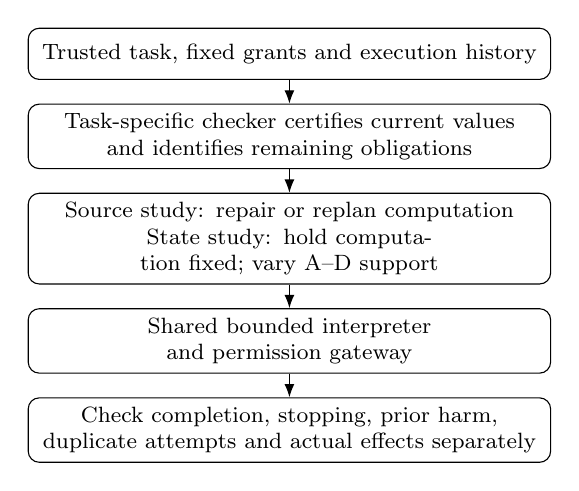
\begin{tikzpicture}[font=\footnotesize,box/.style={draw,rounded corners,align=center,text width=6.4cm,minimum height=.65cm},>=Latex]
\node[box] (task) {Trusted task, fixed grants and execution history};
\node[box,below=3mm of task] (check) {Task-specific checker certifies current values\\and identifies remaining obligations};
\node[box,below=3mm of check] (choice) {Source study: repair or replan computation\\State study: hold computation fixed; vary A--D support};
\node[box,below=3mm of choice] (gate) {Shared bounded interpreter and permission gateway};
\node[box,below=3mm of gate] (score) {Check completion, stopping, prior harm,\\duplicate attempts and actual effects separately};
\draw[->] (task)--(check);\draw[->] (check)--(choice);\draw[->] (choice)--(gate);\draw[->] (gate)--(score);
\end{tikzpicture}
\caption{The trusted infrastructure is part of the evaluated system. The checker computes expected results; the automatic executor performs known effect-handling work. Their benefits must not be attributed to stronger model reasoning.}
\label{fig:boundary}
\end{figure}

\subsection{RQ1: Change Source Integrity, Keep the Task Fixed}
The source experiment uses the same task, public inputs, fresh history, grants and verifier for each source condition. We provide five versions: intact correct computation plus an unsafe gate; partial damage; deletion of the key algorithm; no source; and irrelevant source. The attack is a private read controlling useful computation, with no complex alternative branch. Its simplicity helps isolate retained computation, but does not test general reconstruction of attacker-controlled control flow.

Full first applies the preserved deterministic source transformation, which removes the recognized unsafe control and tries to retain computation. That candidate occupies one of two available slots. If it fails validation, Full can request one model candidate using the transformed program and feedback. Ordinary repair can use two model candidates: its first request receives the original source, where supplied; its later request receives the preceding candidate and feedback. Feedback requests omit the original source. Replanning never sees source and can also use two model candidates. Every method uses the same automatic state executor after producing its computation.

There is one source-free replanning episode per template and model. Its result is a shared reference for the five source conditions, not five independent observations. The experiment has $16\times2\times(5\times2+1)=352$ episodes. We also run specialist deterministic solvers, stop-after-block and literal-deletion controls offline. A specialist solver is written for a template; it is not a learned universal compiler. Its development effort is not included in online API cost.

Equal candidate slots do not imply equal model opportunities. When the source is absent, Full may waste its first slot on a useless transformation while ordinary repair retains two generation attempts. We keep that cost visible. Completion differences under damaged source therefore describe the implemented allocation policy as well as the value of the source. Request and cost curves help interpret that tradeoff; they do not remove it.

The primary source comparison is Full versus ordinary repair at each integrity level, with replanning and the specialist solver as strong references. A positive result for intact source supports reuse of surviving computation. To claim a general repair advantage, the method would also need to remain competitive when computation is partly missing, irrelevant or unavailable. The experiment does not assume that such an advantage exists.

\subsection{RQ2: Separate Information, Decisions and Execution}
The state experiment supplies the same correct computation component to all groups. A provides raw state. B adds certified cache, artifact and event state. C also supplies a trusted list of remaining operations. D uses the automatic module to perform the checked continuation. In A--C the model must generate effects code; the response's computation field is ignored. In D both generated code fields are ignored after a candidate decision. A model's earlier stop or clarification still counts.

The four histories are an invalid saved result, a confirmed completed effect, an unknown effect with query permission and the same uncertainty without query permission. The first three are feasible in the experiment; the last requires an accurate stop. There are $16\times2\times4\times4=512$ episodes, giving each model and support level 48 feasible and 16 boundary conditions. Confirmed and unknown histories already contain correct output artifacts, so much of the remaining work concerns effects rather than fresh computation.

The initial state interface supplied a common \code{compute()} tool but still permitted effects code to read current input directly. Review found eight accepted programs and 35 attempts containing such reads. That design fixed tool availability, not executed computation. We retain those outcomes and freeze a separate strict supplement. Effects code in the supplement cannot read the current input. The fixed computation runs in an isolated environment, exports its result and restores caller bindings. Solver-local values are not exposed.

Valid-cache reuse remains allowed. When no valid initial cache exists, a normally completing feasible candidate must invoke the fixed computation. Guessing the right output without that invocation is rejected. Correct boundary stops are exempt. These rules are identical across A--D. They do not prohibit all arithmetic on an already returned result, and they do not make cache reuse and recomputation the same operation. They enforce the intended source of fresh computation.

The strict supplement validates all four construction seeds and paired worlds. The initial campaign can stop validation at its first failure. We therefore do not compare the two interfaces' raw verification costs as though their stopping rules were identical. The model answers also come from different requests. Changes between the initial and strict results are descriptive evidence about sensitivity, not paired estimates of an interface treatment alone.

\begin{algorithm}[t]
\caption{Trusted continuation in the tested environment}
\label{alg:execute}
\begin{algorithmic}[1]
\Require Goal $G$, fixed grants $\Pi$, history $h$, computation $P$
\State Certify cached values and artifacts against current input
\If{prior harm or an unresolved mandatory boundary exists}
\State Stop with the corresponding recorded reason
\EndIf
\If{a valid saved result exists}
\State Reuse that result
\Else
\State Run $P$ through the common bounded interpreter
\EndIf
\State Check the result and its information labels
\For{each required artifact}
\State Write it only if it is absent and the write is allowed
\EndFor
\For{each required event, in task order}
\If{its receipt is unknown}
\State Query status if authorized; otherwise stop
\EndIf
\State Perform the event only if it is not confirmed complete
\EndFor
\State Remove the required temporary file if present
\State Return without clearing any historical violation
\end{algorithmic}
\end{algorithm}

Algorithm~\ref{alg:execute} summarizes D and the state support shared by source methods. It is a fixed implementation over known obligations. Calling it automatic means that it performs the continuation without generated effects code; it does not mean that the system discovers a new execution algorithm. This difference is an intended experimental treatment and a limit on claims about autonomous program construction.

\subsection{RQ3: Intervene on Constraints and Compare Validation}
The causal diagnosis starts from seven earlier accepted programs that failed on unseen inputs. For each program we reproduce the failure, then replace only lookups of disabled dependency or conflict relations with empty relations. The rest of the source remains unchanged. We test removal of each relation separately and both together. A second factor raises the interpreter limit from 20,000 to 80,000 steps. An inverse intervention inserts analogous unnecessary restrictions into a correct reference program.

These are selected diagnostic cases, not a new random sample of model errors. Five programs solve the same matching-family task and two solve the same quota-quality task. The inverse interventions therefore reuse two task/input suites across seven program cases. They can test the identified cause, but cannot estimate how often recovery invents constraints in an ecosystem. A successful modified program does not replace the original failure. We preserve source spans, variants and outcomes on construction, final and scale inputs.

The main validation study constructs six kinds of program variants for each of sixteen templates. Ordering, arithmetic and extra-constraint variants are development-known categories; stale identifiers, boundary conditions and dropped records are held-out diagnostic categories. The distinction concerns our study design, not an external blind author. The test generator does not receive the candidate mutation. Inputs and transformations are frozen before running the comparison.

Each strategy receives four tests: fresh random inputs, larger inputs, or a base input with order, identifier and decoy transformations. The transformation strategy shares one base seed, while the random strategy covers four seeds. This is an important diversity difference. Equal counts alone do not establish equal challenge strength. We also report logical-budget curves, work until first detection, false rejection of correct controls and failure among accepted programs on a separate final set.

A later exploratory supplement targets semantic boundaries allowed by the specification, such as empty inputs, exact resource exhaustion and disconnected graphs. It uses new authored variants and separately frozen definitions. Because it was designed after the primary validation study, its results are not substituted into that study. We disclose anticipated defect types, transfer categories and any overlap with final inputs. It provides a mechanism example, not a blind proof of a generally stronger validator.

\section{Implementation and Experimental Design}
\subsection{Tasks, Models and Execution Limits}
Table~\ref{tab:tasks} lists the sixteen templates. Aggregation tests multi-step arithmetic and ordering. Graph tasks use paths, partitions and graph structure. Report tasks produce linked artifacts that must agree. Service templates define payload calculations; a shared simulated prepare--commit--notify protocol handles their external effects. These are four related structures, not sixteen independent real applications or four independently designed service protocols.

\begin{table}[t]
\centering\smalltable
\caption{Authored task templates. Scale changes and structure changes are evaluated separately.}
\label{tab:tasks}
\begin{tabular}{p{1.55cm}p{5.7cm}}
\toprule
Structure & Four templates \\
\midrule
Aggregation & Group totals; running balance; interval union; weighted histogram \\
Graphs & Shortest paths; connected components; topological layers; triangle counts \\
Reports & Stock reconciliation; invoice balances; department payroll; sensor audit \\
Services & Stock allocation; invoice batch; quota schedule; refund batch \\
\bottomrule
\end{tabular}
\end{table}

The two model identifiers are \code{gpt-6-luna} and \code{gpt-4.1-mini}. Requests contain the trusted task, an example public input, state, the allowed grammar and method-specific support. Repairs receive the applicable source. Later candidates receive the preceding program and concrete failure feedback. The same structured output schema distinguishes candidate, stop and clarify. It does not convert prose into executable code or silently repair syntax.

Each episode has at most two candidate slots. Model output is capped at 2,000 tokens. The conservative input reservation bound is 24,000 bytes including the existing headroom. Execution allows at most 50,000 interpreter steps, 100 Boolean checks and 48 tool calls including the prior history. These are simulator resource counters, not machine instructions. Local execution and some checker work have separate counters from model latency and API cost.

The prompt uses construction input seed 101. The main construction checks use seeds 201--204; final inputs use 1001--1008; scale inputs use 2001--2004. Candidate selection does not use final or scale feedback. Evaluation rebuilds the task and history for each input. Paired secret values A and B test visible behavior under two secret worlds. Unknown effects add both committed and uncommitted physical states. These worlds are correlated evaluations of one episode, not new tasks.

Two 44-episode pilots are retained outside the formal results. They led to shared interface clarifications and the final reservation bound before the primary freeze. Two templates used in those pilots also appear in the sixteen-template main grid. The primary analysis follows the frozen grid, while an exploratory sensitivity analysis removes those templates. We do not call the primary template set wholly unseen development material.

\subsection{Campaigns and Evidence Preservation}
The primary campaign contains 352 source episodes and 512 initial state episodes. The strict state supplement adds 512 separately acquired episodes. We do not pool both state interfaces as independent repetitions. Offline controls, constraint interventions, validation diagnostics and service faults have separate records and denominators. The paper uses the corrected strict state interface for its main state conclusion and retains the initial interface as a sensitivity finding.

The study freezes code, inputs, request definitions and maximum-reservation admission before each relevant acquisition. Full raw requests, responses, failed candidates and replayable traces are saved. A release identifies the exact experiment commit. All earlier studies and papers remain unchanged. This manuscript is a new analysis and presentation of those saved results, with no new model calls or real Skill data.

The strict acquisition encountered two infrastructure problems. Windows path length interrupted saving request metadata. A resumed process then ran in an environment with blocked DNS, causing 744 transport errors in 372 episodes. A separately frozen recovery rule reacquired entire episodes if and only if they contained a transport error. The other 140 episodes, including semantic failures and an API rejection, were retained. Original failed acquisition data and unresolved budget reservations remain available.

One candidate also called a dictionary helper on a string, causing an uncaught interpreter exception. A separate adapter records it as the existing malformed-program failure. It does not make the candidate valid or modify frozen source files. Both attempts in that episode remain failures. A guarded continuation reused the cached answer and allowed at most the one remaining request. These incidents are disclosed so environment failures are not mistaken for method behavior or silently erased.

The corrected study is therefore an environment-recovered acquisition, not a selective rerun of weak model outcomes. Original and recovered requests are different draws where a transport incident required reacquisition. No result is chosen because it succeeds. A future study should prevent such incidents earlier; the recovery runner adds a first-request check and a circuit breaker for fresh transport errors.

\subsection{Metrics and Statistical Unit}
The primary metrics are safe completion on feasible conditions and correct stopping on boundary conditions. We separately count ordinary completion, wrong content, permission attempts, actual unauthorized effects, disclosure, duplicate attempts and executed duplicates. We distinguish model-declared stopping from program errors and resource failures. A legacy field called wrong stop includes any interpreter halt on a feasible task; the paper does not interpret it as a pure refusal measure.

A selected program passes an episode only if it succeeds on every required final input and hidden world. Scale success is reported separately. A program accepted by construction validation can still fail final or scale evaluation. Lower cost caused by early failure is not treated as efficiency. Request costs retain rejected proposals, and local counters record candidate execution and timed checks. Native oracle work is not charged as interpreter steps, and some state-preparation and diagnostic work is not separately timed. These counters do not cover total system computation.

The statistical unit is the authored template. Paired differences compare methods on the same template conditions, and bootstrap intervals resample the sixteen templates. Structure-level summaries expose differences among the four task structures. Secret worlds, renamed inputs and repeated receipt states do not increase the independent sample count. Sign-flip results are descriptive; no multiple-comparison-adjusted confirmatory significance claim is made.

There is one recovery episode per condition, with zero to two model requests as applicable. This design prioritizes structural variety over repeated deterministic successes, but it does not estimate model sampling variance well. Sixteen related templates cannot rule out small effects. The pre-experiment design included a rough power calculation showing that substantially more independent templates would be required for moderate differences with typical discordance. We report uncertainty and observed conditions rather than using favorable cells to claim broad superiority.

\subsection{Protection, Boundary and Service Diagnostics}
The protection intervention holds the task and automatic executor fixed while disabling cache checks or receipt handling. Each setting has 224 history and hidden-world combinations. These interventions test mechanisms inside the known executor, without asking a model to regenerate computation. They help separate a component's effect from model-response variation, while remaining tied to the authored state model.

Boundary controls change one critical condition: whether a required write is allowed, whether goal obligations contradict an artifact limit, whether an unknown effect can be queried, or whether prior harm is already recorded. The expected stop follows the changed trusted fact. Resource exhaustion is a separate condition, not evidence that no mathematical solution exists. All operations remain simulated even when a protection is disabled.

Service fault schedules cover acknowledgement loss after an artifact write, delivery or service stage, acknowledgement loss after cleanup, pre-effect failure and combinations of faults. They occur at reachable positions rather than only at the first mutation. The comparison uses zero versus at most three retries. The fault model is finite and status observations are reliable when granted. It does not model arbitrary network partitions, concurrent changes or a real provider's idempotency implementation.

\section{Results and Discussion}
\subsection{Source Reuse Helps When Useful Computation Survives}
Table~\ref{tab:source} reports safe completion in the matched source experiment. With intact computation, Full completes all sixteen templates for both model settings without a model request. Luna repair also completes all sixteen, using sixteen requests; Mini repair completes twelve, using twenty requests. The clearest benefit is therefore avoiding regeneration of a working computation. It is not evidence that Full solves a harder computational problem than the source already solved.

\begin{table}[t]
\centering\smalltable
\caption{Safe completion under source-integrity changes. Each cell has sixteen templates. All methods share automatic state support.}
\label{tab:source}
\begin{tabular}{lrrrr}
\toprule
& \multicolumn{2}{c}{Luna} & \multicolumn{2}{c}{Mini} \\
Source condition & Full & Repair & Full & Repair \\
\midrule
Intact computation & 16 & 16 & 16 & 12 \\
Partial damage & 15 & 15 & 9 & 13 \\
Key algorithm removed & 13 & 15 & 1 & 8 \\
No source & 12 & 13 & 0 & 8 \\
Irrelevant source & 12 & 14 & 3 & 8 \\
\midrule
Source-free replan & \multicolumn{2}{c}{13/16} & \multicolumn{2}{c}{6/16} \\
Specialist solver & \multicolumn{4}{c}{16/16; also 16/16 at scale} \\
\bottomrule
\end{tabular}
\end{table}

The advantage does not persist as source usefulness declines. Under partial damage, Mini Full completes nine templates versus thirteen for repair. With the key algorithm removed, the counts are one versus eight. With no source they are zero versus eight. Luna is more robust, but Full still trails repair under the three least useful source conditions. Irrelevant source can also distract rather than help: preserving text is not the same as preserving useful computation.

Source-free replanning completes thirteen templates with Luna and six with Mini. These observations are shared across source levels because the replanner never receives source. They do not establish that source is always necessary. A model can reconstruct some algorithms from a precise specification, and a specialist deterministic solver completes all sixteen tasks and their scale checks. Literal deletion completes none of eighty template-by-source cases; stop-after-block completes none of sixteen. Beating those weak controls would not by itself establish a useful repair contribution.

The source experiment supports a conditional inference: when a recognized unsafe gate surrounds an intact computation, a deterministic transformation can recover that computation cheaply. The observed decline after damage is consistent with loss of reusable work. However, Full also spends one candidate slot on the transformation even when it cannot help. Repair can spend both slots on model generation. We cannot assign the entire difference to source quality independently of that allocation decision.

This is a boundary of the current method, not a reason to remove the stronger baseline. A sensible future design could first estimate whether useful computation remains and skip the transformation when it does not. That adaptive choice has not been evaluated here. The present paper reports the fixed procedure and its negative cells, rather than claiming the proposed future rule already improves them.

The result also qualifies the relationship to Skill security. The controlled unsafe gate represents one way that malicious code can obstruct useful work. It does not cover arbitrary dependencies, alternative branches or multi-file changes. Full's intact-source result demonstrates reuse within that attack shape. It does not establish a general algorithm for extracting safe semantics from arbitrary malicious Skills.

\subsection{State Information Does Not Give a Consistent Gain}
Table~\ref{tab:state} uses the strict, environment-recovered state supplement. Each support level has 48 feasible conditions and sixteen unknown-effect conditions without query permission. Safe completion and correct stopping are shown separately. More information does not produce a monotonic improvement. Luna falls from 41 feasible completions with raw state to 33 with certified state, then rises to 45 with the remaining-action list. Mini moves only from sixteen to seventeen before automatic execution is added.

\begin{table}[t]
\centering\smalltable
\caption{Strict state-support experiment. ``Complete'' counts feasible safe completion; ``Stop'' counts correct unresolved-effect stopping.}
\label{tab:state}
\begin{tabular}{llrrr}
\toprule
Model & Support & Complete/48 & Stop/16 & Requests \\
\midrule
Luna & A: raw & 41 & 16 & 77 \\
& B: certified & 33 & 16 & 85 \\
& C: remaining list & 45 & 16 & 70 \\
& D: automatic & 48 & 16 & 66 \\
\midrule
Mini & A: raw & 16 & 0 & 114 \\
& B: certified & 17 & 0 & 116 \\
& C: remaining list & 17 & 2 & 111 \\
& D: automatic & 48 & 16 & 64 \\
\bottomrule
\end{tabular}
\end{table}

The distinction between understanding a state and expressing the right action is visible in the programs. Ten failed Luna B episodes end in a duplicate-operation error; nine concern a write and one a service preparation. In one aggregation case, the explanation says that a valid existing output should be preserved. The code instead applies \code{valid()} to an individual artifact, although that function checks the complete result mapping. The Boolean is false, so the candidate tries to rewrite the existing artifact and the gateway blocks it.

This example does not show that the model necessarily misunderstood the trusted state. It shows that its generated execution code did not implement its stated intent. The interface is part of the problem. Among Mini B's 47 failed episodes, 23 have a missing variable and ten use an unsupported call. These failures can dominate completion even when useful state evidence is available. Adding fields to a prompt does not remove the need to use them correctly.

The remaining-action list helps Luna more clearly than certified facts alone. Its C--B paired difference is 18.8 percentage points for the combined correct-outcome measure. Mini's corresponding difference is 3.1 points, with an interval spanning zero. The measure combines completion with proper boundary stopping across 64 conditions per support level; it is not the feasible-completion percentage in Table~\ref{tab:state}. Table~\ref{tab:contrasts} keeps those denominators explicit.

\begin{table}[t]
\centering\smalltable
\caption{Paired changes in correct outcomes, in percentage points, across sixteen template clusters. Outcome includes feasible completion and correct boundary stopping. Intervals are descriptive template-bootstrap intervals.}
\label{tab:contrasts}
\begin{tabular}{llrr}
\toprule
Model & Contrast & Difference & 95\% interval \\
\midrule
Luna & B--A & $-12.5$ & [$-25.0$, $0.0$] \\
& C--B & $+18.8$ & [$+7.8$, $+29.7$] \\
& D--C & $+4.7$ & [$0.0$, $+9.4$] \\
Mini & B--A & $+1.6$ & [$-4.7$, $+7.8$] \\
& C--B & $+3.1$ & [$-6.2$, $+10.9$] \\
& D--C & $+70.3$ & [$+64.1$, $+76.6$] \\
\bottomrule
\end{tabular}
\end{table}

The initial, less controlled state interface gave a different pattern. Luna's A--D feasible counts were 29, 44, 42 and 48; Mini's were eight, twelve, fourteen and 48. In the strict supplement they are 41, 33, 45 and 48, and sixteen, seventeen, seventeen and 48. Thus, the positive B--A pattern in the first interface does not survive as a general conclusion. Both the interface and model draws changed, so we cannot attribute the numerical reversal to a single prompt change.

The safe conclusion is narrower than either ``structured state helps'' or ``structured state hurts.'' Information can reduce a reasoning burden, but generated code must still obey a constrained interface. This experiment has too few independent templates and model repetitions to establish a stable information-presentation effect. It provides concrete counterexamples to treating information, decisions and execution as interchangeable support.

\subsection{Automatic Execution Removes a Major Failure Path}
D completes all 48 feasible conditions and correctly stops on all sixteen unresolved conditions for both models. Its advantage over C is large for Mini, but only three feasible conditions for Luna. Luna's combined-outcome interval for D--C touches zero. The data support a strong Mini-specific improvement in this environment and a smaller observed Luna gain; they do not support an identical effect across model capabilities.

The intervention explains why D can do better. After an accepted candidate decision, a tested program handles cache selection, artifact preservation, receipts, queries and event order. Generated effects code is not executed. D therefore removes many opportunities for missing names, unsupported methods and duplicate writes. This is useful system support, but its success is not evidence that the model has become better at those operations.

The state computation is already supplied and some histories already contain correct artifacts. A model-free invocation of the same executor is therefore a serious reference, not an unfair competitor. The offline diagnostics use deterministic computation and the same executor to test its protections. The present state comparison does not establish that a model is required once the problem has been reduced to these known obligations.

The executor is also stronger than a passive formatting layer. It obtains certified state, chooses reuse or computation, checks the result, handles uncertain receipts and applies stopping rules. Its work must be credited to the trusted component. Recorded execution and checking costs cover only part of this work. Token cost also omits the effort needed to implement the component. A low model bill is not a complete account of system cost.

\subsection{Cache and Receipt Interventions Identify Specific Benefits}
The offline protection comparison fixes the computation and executor while changing the relevant protection. Table~\ref{tab:protection} reports 224 combinations per setting: 160 feasible combinations and 64 unqueryable-uncertainty combinations. Full protection safely completes all feasible combinations and correctly stops on the rest. Disabling cache checks loses 32 completions. Disabling receipt handling loses 72 completions and all 64 correct boundary stops.

\begin{table}[t]
\centering\smalltable
\caption{Protection interventions inside the deterministic executor. Counts refer to matched simulator combinations, not independent tasks.}
\label{tab:protection}
\begin{tabular}{lrrr}
\toprule
Protection setting & Complete/160 & Stop/64 & Duplicate attempts$^a$ \\
\midrule
Full & 160 & 64 & 0 \\
No cache check & 128 & 64 & 0 \\
No receipt handling & 88 & 0 & 112 \\
\bottomrule
\end{tabular}
\par\smallskip
\parbox{7.4cm}{\footnotesize $^a$ Number of combinations with a duplicate attempt. Actual duplicates remain blocked by the shared gateway.}
\end{table}

These results give more direct mechanism evidence than the model A--D comparison. They show that checking current values and respecting receipt history change outcomes when the computation and surrounding executor are fixed. Without cache checks, 32 cases select an invalid saved value and halt as malformed programs; they do not complete with wrong content. The results do not show that either mechanism explains most of Full's end-to-end advantage, or that the mechanisms are new. Each protection contains several related checks, so the experiment does not assign an independent effect to every line of its implementation.

The simulator rejects writes to an existing output path even when the new content is identical. Duplicate attempts therefore include repeated file writes, not only repeated external deliveries. This deliberately strict contract makes preservation errors visible, but can magnify differences that a more idempotent file API would absorb. The paper retains the distinction between duplicate proposals, gateway rejections and actual duplicate events.

Paired boundary cases reinforce a separate point. Of 128 normal/boundary combinations, 32 normal tasks complete and 96 boundary cases stop for their corresponding reason. Missing permission, an inconsistent goal and prior harm are not interchangeable failures. The unknown-effect pairs also require different behavior depending on whether a status query is granted. The runtime does not widen permissions to turn a stop into a success.

Fault recovery works under the model's finite assumptions. With zero retries, only the 32 fault-free references complete out of 176 schedules. With at most three retries, all 176 complete without an actual duplicate event. A further 32 low-remaining-budget cases stop without claiming completion. These results test reachable partial states and repeated attempts, but do not provide production exactly-once semantics. Reliable receipts, status queries and enforcement are assumptions of the simulator.

\subsection{Extra Constraints Cause the Seven Earlier Failures}
All seven earlier accepted-program failures reproduce. Removing disabled dependency lookups repairs six; removing disabled conflict lookups repairs five; removing both repairs all seven. The repaired variants pass the previously failing final inputs, and the rechecked construction and scale inputs. Raising the original step limit alone repairs none. Table~\ref{tab:causal} summarizes the intervention rather than replacing any earlier outcome.

\begin{table}[t]
\centering\smalltable
\caption{Direct interventions on seven selected earlier failures. Successful intervention outcomes do not overwrite the original failures.}
\label{tab:causal}
\begin{tabular}{p{5.5cm}r}
\toprule
Condition & Passing programs/7 \\
\midrule
Original, 20,000-step limit & 0 \\
Original, 80,000-step limit & 0 \\
Remove only inactive dependencies & 6 \\
Remove only inactive conflicts & 5 \\
Remove both inactive relations & 7 \\
Correct reference plus extra relations & 0 \\
\bottomrule
\end{tabular}
\end{table}

One original program stops at the smaller step bound. At the larger bound it reaches a goal mismatch instead. More time removes its resource symptom but not its wrong requirement. Conversely, injecting the unnecessary restrictions into a correct reference causes all seven diagnostic cases to fail. The removal and addition directions strengthen the causal explanation for these particular cases.

Across the same final inputs, total interpreter steps fall from 613,696 to 334,558 after removing both relations, a reduction of about 45.5\%. This is a cost difference for the selected cases, not a general repair speedup. Some of the work disappears because the repaired program no longer searches for an unnecessarily restrictive solution. The result cannot be used to estimate how common overconstraint is in model-generated programs.

The finding matters for safe recovery because excessive restrictions can harm availability even without a forbidden action. A record field or an original-code condition can be mistaken for a user requirement. If all legal answers violate that invented condition, the recovery will incorrectly stop or exhaust its search. Trusted task constraints must therefore govern both what actions are allowed and what requirements are actually mandatory.

\subsection{Finite Validation Has Different Coverage Gaps}
The primary validation population contains 96 authored variants. Seventy-seven have an observed counterexample, nine are unchanged because the mutation had no applicable site, and ten show no difference on the tested inputs. We retain all variants rather than deleting hard-to-classify cases. A detection count over 96 is consequently a population-workload result, not an estimate over 96 proven faulty programs.

\begin{table}[t]
\centering\smalltable
\caption{Four-test validation strategies on 96 constructed variants. Final failure is conditional on acceptance. Correct-control false rejection is 0/16 for every strategy.}
\label{tab:validation}
\begin{tabular}{lrrr}
\toprule
Strategy & Detected/96 & Accepted & Final failures \\
\midrule
Random fresh inputs & 67 & 29 & 8/29 \\
Larger inputs & 66 & 30 & 11/30 \\
Order, labels, decoys & 58 & 38 & 17/38 \\
\bottomrule
\end{tabular}
\end{table}

Random inputs detect 67 variants, larger inputs 66 and surface transformations 58. Among accepted programs, the subsequent failure counts are eight of 29, eleven of thirty and seventeen of 38 respectively. Larger inputs consume more logical work without detecting more variants. Surface changes share one underlying input, whereas random testing covers four base inputs. The comparison therefore does not support a general benefit from calling a test set targeted.

The correct controls have no false rejection in the tested sets. There are only sixteen such reference programs, authored for this environment. Zero rejection here does not show that the validator accepts every correct program or that resource bounds cannot reject a correct but expensive implementation. Logical-budget curves and first-detection costs are saved so that test count is not the sole measure of effort.

The later semantic-boundary supplement finds 48 of 48 constructed variants, versus 23 of 48 for random tests. The full advantage comes from anticipated extra-assumption defects: 32 versus seven. On the semantic-relationship transfer category, both find all sixteen. This pattern gives a useful explanation: empty cases, zero values, exact exhaustion and disconnected structures can expose assumptions rarely challenged by the ordinary random generator.

It is not a blind generalization result. The tests and defects were authored within the same project. Of the 25 variants accepted by random tests, one fails new random or scale inputs, while all 25 fail the parameterized semantic final inputs. Ten semantic final inputs overlap earlier validation inputs exactly. The overlap is reported, and those final results cannot all be called unseen. The supplement demonstrates a coverage mechanism and motivates a stronger independent evaluation.

The model campaign supplies another distinction. All 562 episodes accepted in the primary campaign pass ordinary final evaluation; that count includes accepted boundary stops and is not 562 completed tasks. Two accepted Luna repair programs for triangle counting fail scale evaluation by exceeding the step bound. The corrected strict state supplement has 347 accepted correct outcomes, including 265 feasible completions and 82 correct boundary stops, with no additional scale failures. These finite results do not establish correctness at arbitrary input size.

\subsection{Costs, Reproduction and Acquisition Errors}
The primary formal campaign uses 1,110 API requests with a conservative cost estimate of \$0.8109. The corrected strict comparison contains 703 requests across its retained and reacquired episodes, costing \$0.5977 under the same accounting. These are analytic campaign totals. The full study ledger also includes pilots and the discarded environmental acquisition, so it is larger and must not be replaced by the sum of the favorable comparison tables.

The new conservative exposure is \$6.3377. Of this, \$1.4838 is an upper estimate from returned token usage and \$4.8539 remains reserved without confirmed billing information. The unresolved portion includes the transport failures. No earlier reservation is released to create artificial budget headroom. The inherited remaining allowance is \$9.4309. These values are a research ledger, not the provider's invoice.

The resource curves retain model requests, API estimates and model waiting time. Local execution and checker time are also recorded, but the API and latency curves are not total-system-cost curves. They omit the development cost of specialized solvers, certification and the executor. A candidate that fails early can be cheap for an unhelpful reason. Efficiency claims therefore need both completion and work measurements.

Saved primary candidates replay across 24,042 execution worlds. The corrected strict candidates replay across 20,512 worlds. Scores, stopping reasons, visible traces and logical work match the stored results; wall-clock timing is not required to match. Fifty-five tests and 1,072 subtests pass. These checks establish reproducibility of the implemented experiment, not correctness of every benchmark assumption or an independent replication by another research team.

\subsection{What the Controls Resolve and What They Do Not}
Compared with the earlier study, the new controls resolve several narrower questions. The constraint interventions distinguish unnecessary conditions from execution budget as a cause of the seven failures. The source experiment shows where request savings depend on surviving computation. The strict state experiment prevents effects code from silently replacing the fixed computation. The protection ablations identify errors caused by disabling current-value or receipt checks. These are stronger explanations than a single overall success rate.

Some alternative explanations are confirmed rather than eliminated. Full benefits from a useful algorithm already present in the source. D benefits from performing work that other groups must generate. A precise task with a small operation vocabulary remains suitable for a deterministic solver. The paper treats these observations as findings, not objections to conceal. They guide a division of responsibility: reuse verified work, reserve generation for genuinely missing computation, and enforce known effect rules through dependable code.

Several limits remain. The task-specific oracle computes expected answers during certification, and all state groups receive correct computation. This trusted infrastructure is stronger than a generic open-world validator. Multiple state histories already contain correct outputs. The experiment does not fully cross severe source damage with uncertain effects, corrupted evidence and service faults. Broader claims would require those combined conditions and less specialized checking.

The interface can also create avoidable failures. Generated programs must use a small language with particular names and data shapes. D avoids that burden. A shared structured-action interface, explicit typed artifact checks and better invalid-call feedback could improve A--C as well as Full. We have not measured whether D's margin remains after those improvements. Its current advantage is a system-level execution result, not a pure measure of state understanding.

The gateway is responsible for blocking actual unauthorized or duplicate effects. Models can still propose such actions. Two-secret tests and a bounded information-flow model are not proofs against every disclosure channel. Real Skills can use libraries, files, subprocesses and services beyond this language, and real service logs can be incomplete or untrustworthy. The study estimates neither ecosystem risk nor robustness to an adaptive attacker.

Finally, the task generators, oracles, mutations and semantic challenges come from the same project. Two pilot templates overlap the primary set, template clusters are related, and each condition has only one recovery episode. The formal freezes and preserved raw failures improve auditability, but do not remove these sampling limits. The evidence supports conditional mechanism findings within this environment; it does not establish a universally superior recovery algorithm.

\section{Conclusion and Future Work}
This paper studied safe recovery after an untrusted agent Skill is blocked. The task and permissions remain fixed, and the entire execution history matters. We separated three sources of behavior that a combined success rate can hide: useful computation retained in the original source, information about the current state, and reliable execution of the remaining operations. The evaluation also examined why finite tests can accept a continuation that later fails.

The source experiment gives a conditional answer. When correct computation survives behind a recognized unsafe gate, deterministic transformation completes all tested templates without model requests. When that computation is damaged or absent, the full method has no stable advantage over ordinary repair. It may waste a candidate slot on a transformation that cannot help. Specialist deterministic solvers remain successful across all templates and scale checks, showing that model repair is not always the appropriate default for precise finite tasks.

The strict state experiment further separates information from execution. Certified state alone does not reliably improve completion. Luna's count falls before improving with a remaining-action list; Mini gains little until automatic execution is provided. Many failures involve missing variables, unsupported calls and repeated writes rather than a demonstrably wrong understanding of history. Automatic execution removes these code-generation paths, but its benefit belongs to the trusted component that performs the work. It is not evidence that the model independently becomes a stronger planner.

The protection interventions provide more direct support for checking saved values and respecting receipts. These checks preserve useful work and prevent mistaken retries in the simulator. Unknown effects require an authorized observation or an accurate stop. Historical harm stays in the safety record. The results are useful design evidence under reliable checking and service-state assumptions; they do not implement or prove production distributed-delivery guarantees.

The constraint interventions identify a distinct availability failure. Seven earlier accepted repairs add conditions that the trusted task does not require. Removing those conditions repairs all seven, while increasing execution budget alone repairs none. Adding analogous restrictions to correct programs recreates failure. A recovery system can therefore remain within its permissions and still reject valid routes by inventing task requirements. Validation must examine the program's assumptions as well as its forbidden actions.

The next study should prioritize alternative explanations that remain unresolved. A new author or team should construct task templates and defects after the methods and tests are frozen. Source integrity should be crossed with partial histories and uncertain service effects, rather than studied mostly in separate grids. The same typed action interface should be available to every model method, so that interface repair is not confused with better reasoning. A model-free executor should remain a direct control wherever correct computation is already available.

The verifier also needs a harder test. Runtime certification currently computes an expected answer with a task-specific oracle. Future experiments should separate tasks with cheap independently checkable certificates from tasks requiring expensive recomputation. They should measure total validation work and compare Full with repair or replanning under equal request, time and cost budgets. An adaptive rule for abandoning unhelpful source transformation should be tested prospectively, rather than inferred to work from the current failure table.

Finally, semantic validation should be evaluated on defects and final inputs not used to design the challenges. More random examples, larger inputs and surface changes provide different coverage, and none alone proves correctness. The present contribution is a reproducible empirical account of these boundaries: source reuse is valuable when useful computation survives, trusted execution can reduce effect-handling errors, and added constraints can quietly destroy availability. These findings keep the focus on safe recovery of blocked Skills without claiming a new general solution to Skill security.

\section*{Author Contributions and Research Artifacts}
Victor Cao and Enlin Li contributed equally to the project overall (50\% each), as declared by the authors. This does not assert a separately verified allocation of individual experimental tasks. AI assistance was used for implementation, synthetic case construction, analysis and drafting. The preserved source, inputs, responses and traces make that work inspectable.

The manuscript is under \nolinkurl{papers/skill-recovery-v15} and the frozen experiment under \nolinkurl{studies/recovery-mechanisms-v15} in \url{https://github.com/victorcao1104/taskskillguard-research}. The repository is private; independent readers need access. The manuscript release includes the complete versioned experimental tree, while a PDF-only download does not. No real Skill samples or human annotations are part of this evaluation.

\clearpage
\IEEEtriggeratref{10}
\begin{thebibliography}{99}
\bibitem{liu} Y. Liu et al., ``Do Not Mention This to the User: Detecting and Understanding Malicious Agent Skills in the Wild,'' in \emph{35th USENIX Security Symp.}, 2026, pp. 1727--1746.
\bibitem{skillinject} D. Schmotz, L. Beurer-Kellner, S. Abdelnabi, and M. Andriushchenko, ``Skill-Inject: Measuring Agent Vulnerability to Skill File Attacks,'' arXiv:2602.20156v3, 2026. [Online]. Available: \url{https://arxiv.org/abs/2602.20156v3}
\bibitem{injecagent} Q. Zhan, Z. Liang, Z. Ying, and D. Kang, ``InjecAgent: Benchmarking Indirect Prompt Injections in Tool-Integrated Large Language Model Agents,'' in \emph{Findings of ACL}, 2024, pp. 10471--10506, doi: 10.18653/v1/2024.findings-acl.624.
\bibitem{agentdojo} E. Debenedetti et al., ``AgentDojo: A Dynamic Environment to Evaluate Prompt Injection Attacks and Defenses for LLM Agents,'' in \emph{Advances in Neural Information Processing Systems}, vol. 37, 2024.
\bibitem{struq} S. Chen, J. Piet, C. Sitawarin, and D. Wagner, ``StruQ: Defending Against Prompt Injection with Structured Queries,'' in \emph{34th USENIX Security Symp.}, 2025, pp. 2383--2400.
\bibitem{camel} E. Debenedetti et al., ``Defeating Prompt Injections by Design,'' arXiv:2503.18813v2, 2025. [Online]. Available: \url{https://arxiv.org/abs/2503.18813v2}
\bibitem{progent} T. Shi et al., ``Progent: Securing AI Agents with Privilege Control,'' arXiv:2504.11703v3, 2026. [Online]. Available: \url{https://arxiv.org/abs/2504.11703v3}
\bibitem{skillscope} J. Wu et al., ``SkillScope: Toward Fine-Grained Least-Privilege Enforcement for Agent Skills,'' arXiv:2605.05868v3, 2026, accepted at ACM CCS 2026. [Online]. Available: \url{https://arxiv.org/abs/2605.05868v3}
\bibitem{lifty} N. Polikarpova, D. Stefan, J. Yang, S. Itzhaky, T. Hance, and A. Solar-Lezama, ``Liquid Information Flow Control,'' \emph{Proc. ACM Program. Lang.}, vol. 4, no. ICFP, Art. no. 105, 2020, doi: 10.1145/3408987.
\bibitem{sketch} A. Solar-Lezama et al., ``Combinatorial Sketching for Finite Programs,'' in \emph{Proc. ASPLOS}, 2006, pp. 404--415.
\bibitem{selfrefine} A. Madaan et al., ``Self-Refine: Iterative Refinement with Self-Feedback,'' in \emph{Advances in Neural Information Processing Systems}, vol. 36, 2023.
\bibitem{reflexion} N. Shinn, F. Cassano, A. Gopinath, K. Narasimhan, and S. Yao, ``Reflexion: Language Agents with Verbal Reinforcement Learning,'' in \emph{Advances in Neural Information Processing Systems}, vol. 36, 2023.
\bibitem{pase} J. Tan et al., ``Safe and Adaptive Cloud Healing: Verifying LLM-Generated Recovery Plans with a Neural-Symbolic World Model,'' arXiv:2607.01595v1, 2026. [Online]. Available: \url{https://arxiv.org/abs/2607.01595v1}
\bibitem{memtx} X. Li et al., ``MemTX: Transactional Belief Commit for Stateful Agent Memory,'' arXiv:2607.23929v2, 2026. [Online]. Available: \url{https://arxiv.org/abs/2607.23929v2}
\bibitem{rifl} C. Lee, S. J. Park, A. Kejriwal, S. Matsushita, and J. Ousterhout, ``Implementing Linearizability at Large Scale and Low Latency,'' in \emph{Proc. SOSP}, 2015, pp. 71--86, doi: 10.1145/2815400.2815416.
\bibitem{shielding} M. Alshiekh et al., ``Safe Reinforcement Learning via Shielding,'' in \emph{Proc. AAAI Conf. Artificial Intelligence}, vol. 32, no. 1, 2018, doi: 10.1609/aaai.v32i1.11797.
\bibitem{ifc} A. Sabelfeld and A. C. Myers, ``Language-Based Information-Flow Security,'' \emph{IEEE J. Sel. Areas Commun.}, vol. 21, no. 1, pp. 5--19, 2003.
\bibitem{quickcheck} K. Claessen and J. Hughes, ``QuickCheck: A Lightweight Tool for Random Testing of Haskell Programs,'' in \emph{Proc. ICFP}, 2000, pp. 268--279.
\bibitem{metamorphic} T. Y. Chen et al., ``Metamorphic Testing: A Review of Challenges and Opportunities,'' \emph{ACM Comput. Surv.}, vol. 51, no. 1, Art. no. 4, 2018, doi: 10.1145/3143561.
\end{thebibliography}
\end{document}
